\chapter{Flow Patterns and Flow-Pattern Transitions}

Multiphase flow is characterized by the existence of interfaces between the phases and discontinuities of associated properties.
Single-phase flow can be classified according to the external geometry of the flow channel as well as the 'character' of the flow; i.e., laminar - following streamlines, or turbulent - exhibiting fluctuations and chaotic motions.
In contrast multiphase flow is classified according to the internal phase distributions or "flow patterns" or "regimes."
For a two-phase mixture of a gas or vapor and a liquid flowing together in a channel, different internal flow geometries or structures can occur depending on the size or orientation of the flow channel, the magnitudes of the gas and liquid flow parameters, the relative magnitudes of these flow parameters, and on the fluid properties of the two phases.
A wide variety of multiphase flow patterns has been observed and identified in the literature.
For example, Rouhani and Sohel (1983) cited a survey which suggested 84 different flow-pattern labels used in the literature.
These variations are due to the subjective nature of flow-pattern definitions and partly to a variety of names given to essentially the same geometric flow patterns.
In reality one finds a few basic flow patterns with associated transitions.

The rate of exchange of mass, momentum and energy between gas and liquid phases as well as between any multiphase mixture and the external boundaries depends on these internal flow geometries and interfacial area; hence is dependent on flow-pattern.
For instance, the relationships for pressure drop and heat transfer are likely to be different for a dispersed flow consisting of bubbles in a liquid (bubbly flow) than for a separated flow consisting of a liquid film on a channel wall with a central gas core (annular flow).
This leads to the use of flow-pattern dependent models for mass, momentum and energy transfer, together with appropriate flow-pattern transition criteria.
Given the existence of any one pattern, it is possible to model the two-phase flow field and to select a proper set of flow-pattern dependent equations so as to predict the important process design parameters.
However, the central task is to predict which flow-pattern will exist under any set of operating conditions as well as to predict the value of characteristic fluid and flow parameters (e.g., bubble or droplet size) at which the transition from one flow-pattern to another will take place.
Therefore, in order to accomplish a reliable design of gas-liquid systems such as pipe lines, evaporation and condensers, a prior knowledge of the flow-pattern is required.

The common practice in representing flow-pattern data is to classify the flow patterns by visual or other means and to plot the data as a two-dimensional flow-pattern map in terms of particular system parameters.
Beginning with the early flow-pattern maps, such as those proposed by Bergelin and Gazley (1949) and Kosterin (1949), there has been an on-going discussion on the selection of appropriate pairs of parameters to represent the flow-pattern transition boundaries.
There is a wide variety of flow-pattern maps for two-phase flow in channels.
A large number of different parameters have been used to present the experimental data in two-dimensional coordinates based on the superficial velocities, $j_j$ and $j_g$ or $G_j$ and $G_g$.
A good example are the empirical flow regime maps by Baker (1955) for horizontal flow and Hewitt and Roberts (1969) for vertical flow, which are illustrated in Figures \ref{fig:baker_flow_map} and \ref{fig:hewitt_roberts_flow_map}.
Note that both of these maps are for small tubes; i.e., on the order of centimeters.
Some investigators have attempted to correlate the transition boundaries by a single pair of non-dimensional groups, in the hope that the results would apply to pipe sizes, and fluid and flow parameters other than those of the experimental data used to locate curves.
Tables \ref{unk}, \ref{unk}, \ref{unk} and \ref{unk} present suggestions of these parameters together with specific references for their applicability in horizontal and vertical pipe flows.

\begin{figure}[h]
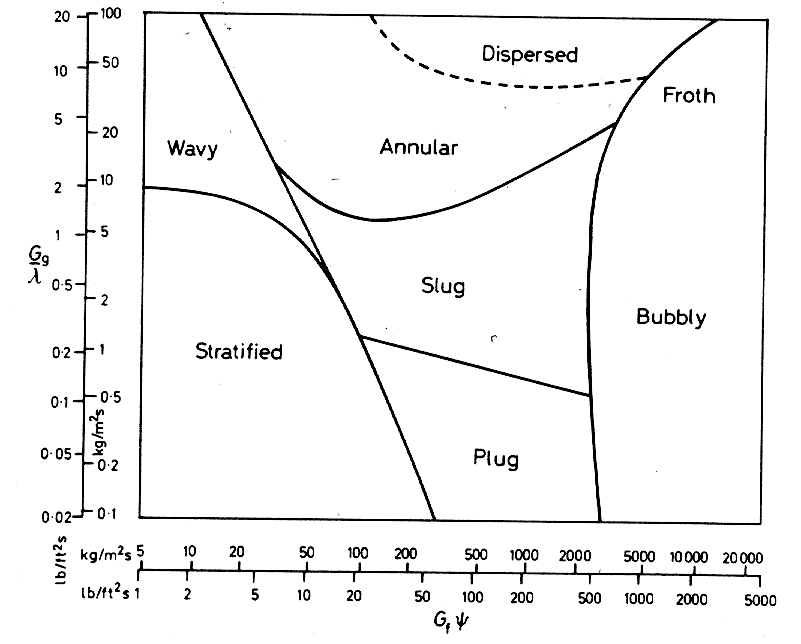
\includegraphics[width=0.5\textwidth]{images/baker_flow_map.png}
\caption{Flow Pattern Map for Horizontal Flow (Baker)}
\label{fig:baker_flow_map}
\end{figure}

\begin{figure}[h]
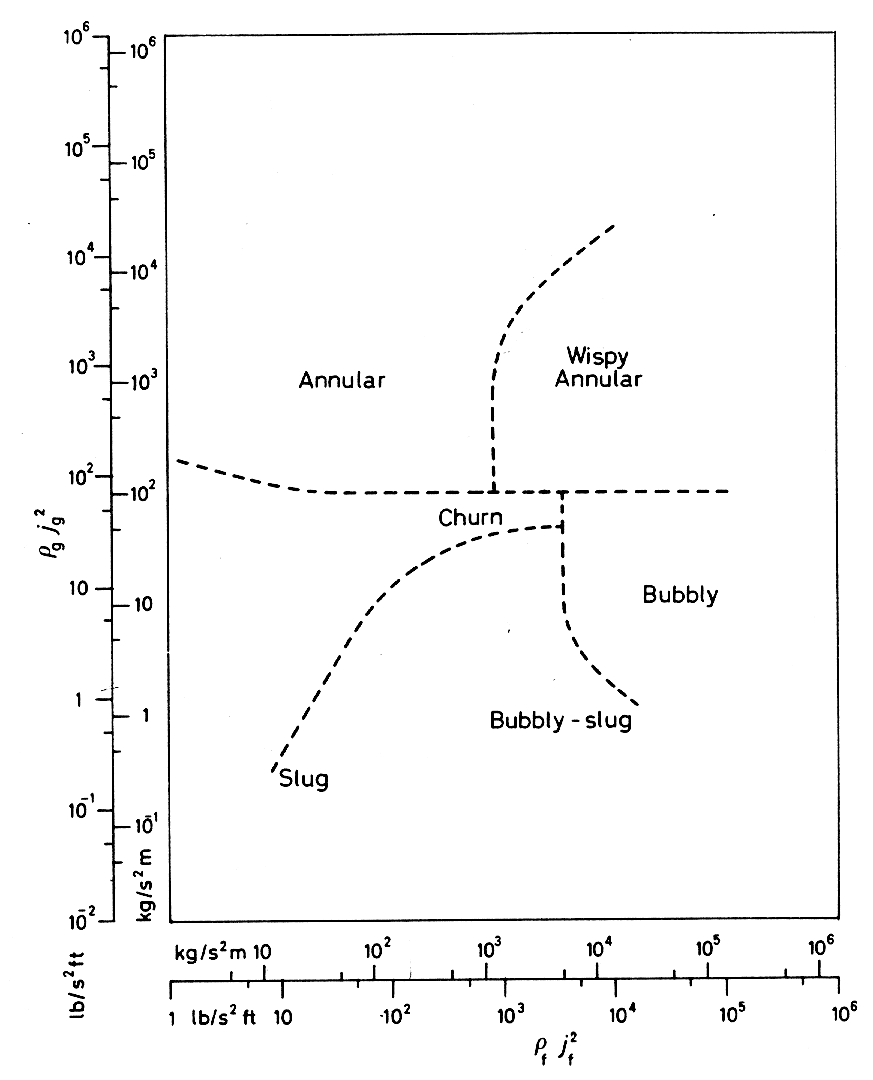
\includegraphics[width=0.5\textwidth]{images/hewitt_roberts_flow_map.png}
\caption{Flow Pattern Map for Vertical Flow (Hewitt and Roberts)}
\label{fig:hewitt_roberts_flow_map}
\end{figure}

The main task is to group together the basic flow structures and define a few basic patterns.
This is by no means well defined and indeed many flow patterns exist as individual researchers group the flow patterns somewhat differently depending on their own interpretations.
Basically the attitude of most practitioners is to minimize the number of flow pattern groups and to group together the flow structures that has basically the same character pertaining to the distribution of the interfaces.
An example of this approach is given in multifluid hydrodynamic models such as TEXAS (Chu, 1986, 1996) where only a bubbly flow or droplet flow is considered for large flow channels (See Figure \ref{fig:texas_flow_map}.).
As noted in the introduction dispersed flow patterns and stratified flow patterns are the two major classifications, with transitional patterns identified between these two groups.\cite{Sheikh1970}

\begin{figure}[h]
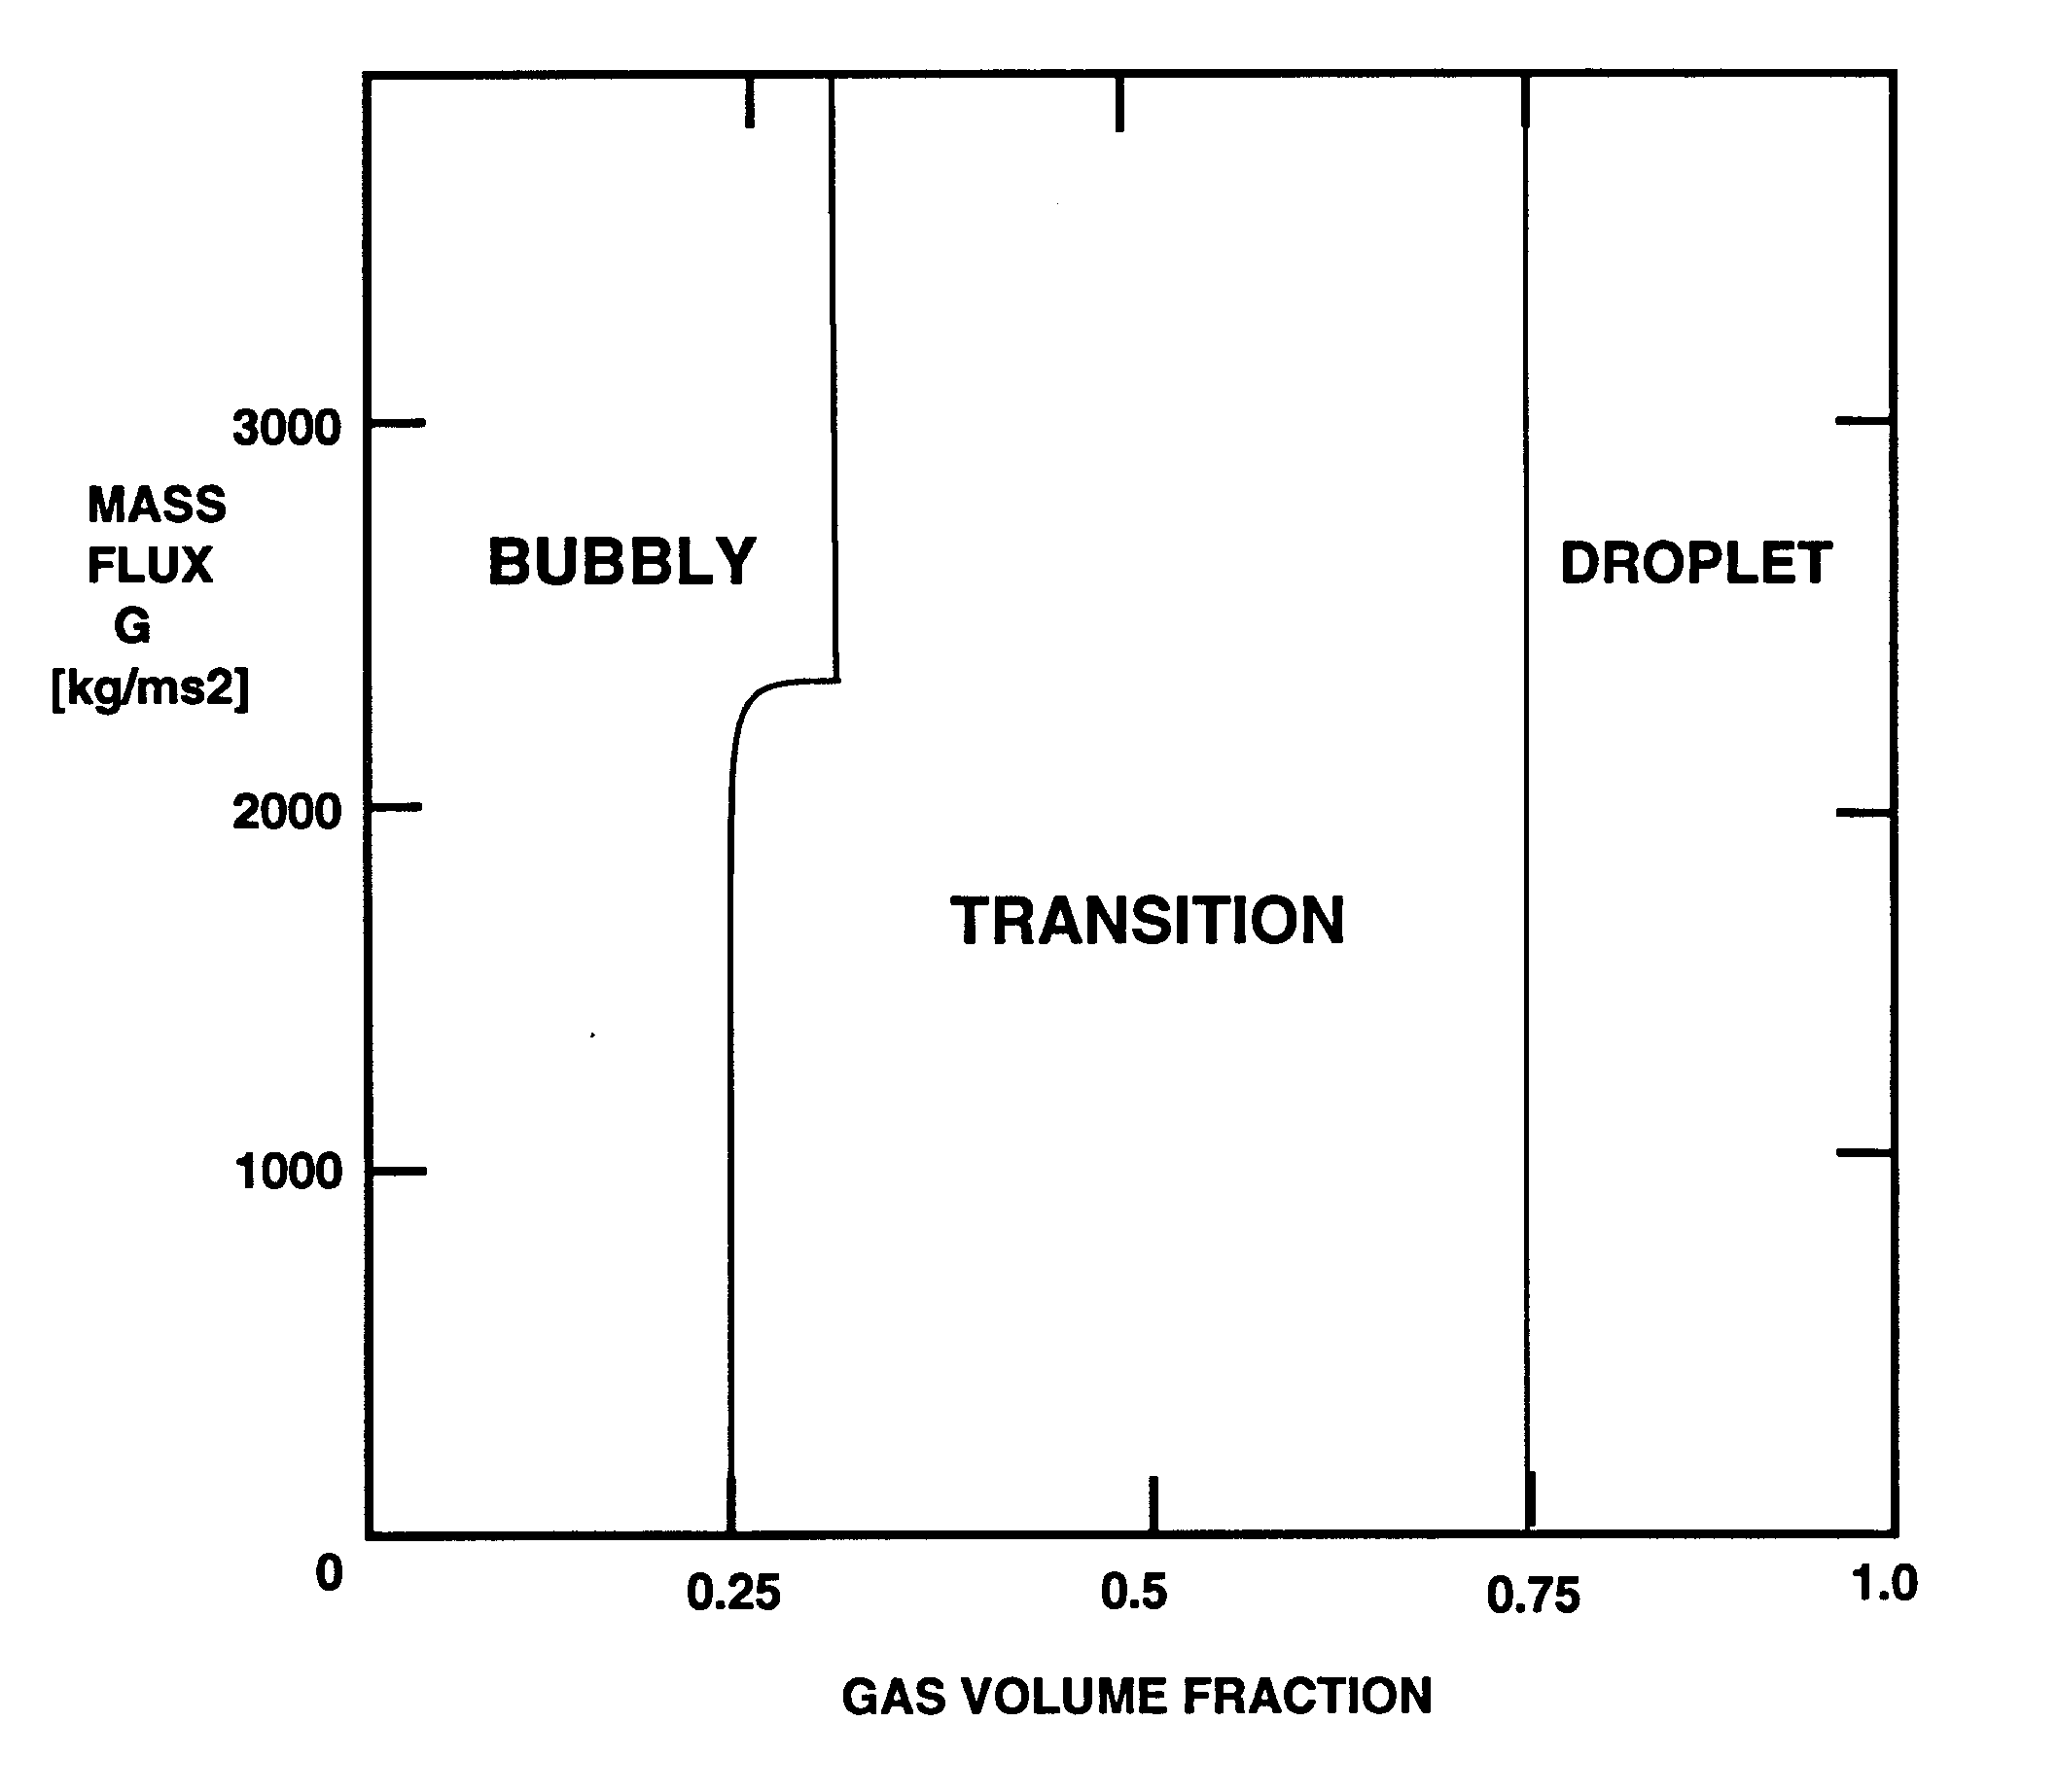
\includegraphics[width=0.5\textwidth]{images/texas_flow_map.png}
\caption{Flow Pattern Map used in TEXAS (Chu)}
\label{fig:texas_flow_map}
\end{figure}



